\documentclass[addpoints,12pt]{exam}
%\documentclass[12pt]{article}
\usepackage[letterpaper, margin=0.75in]{geometry}
\usepackage{graphicx}
\usepackage{enumitem}
\usepackage{booktabs}
\usepackage{tabularx}
\usepackage{color}
\usepackage{wrapfig}

\begin{document}
\footer{}{Page \thepage\ of \numpages}{}

\begin{flushright}
\makebox[0.5\textwidth]{\large Name:\enspace\hrulefill}
\vspace{0.2in}

\end{flushright}

\begin{center}
\includegraphics[width=10cm]{../images/logo.png}
\end{center}

\begin{center}
\noindent{\LARGE Conceptual Physics \\ Second Partial Test\\ \textbf{INDIVIDUAL} \\ May 18, 2018 \\}
\end{center}

\vspace{0.5in}

\begin{large}
You are free to use all notes on your two-sided cheat sheet. There are extra blank sheets at the end, which can be used for calculations, and if you require more please ask and be sure to include them when you hand back the test. Please be sure to include all your work and calculations.

There are \numquestions~problems for a total of \numpoints~points. (One of the questions is a bonus though.)
\end{large}
\vspace{0.2in}


 
\clearpage

\begin{flushright}
Score: \hspace{0.2in} / \numpoints ~ points
\end{flushright}

\begin{questions}
\question \textbf{Drawing Field Lines:} Six particles are arranged on a hexagon. They all have identical masses. Some are positively charged, and some are negatively charged. They all have charge of $\pm 1$ (so the size of all charges are the same).

\begin{parts}

\part[2] Draw the \textbf{electric field} lines around the particles. If there is a point with \textbf{zero} electric field, indicated it on the diagram.
\vspace{1in}
\begin{center}
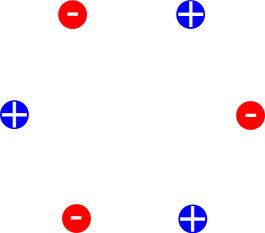
\includegraphics[width=2in]{../images/hexagonCharges.png}
\end{center}
\vspace{1in}

\part[2] Draw the \textbf{gravitational field} lines around the particles. If there is a point with \textbf{zero} gravitational field, indicated it on the diagram.
\vspace{1in}
\begin{center}
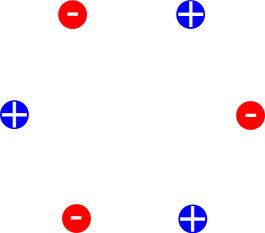
\includegraphics[width=2in]{../images/hexagonCharges.png}
\end{center}
\vspace{1in}
\end{parts}

\clearpage
\question \textbf{Alien Planet:} On a distant planet, aliens have set up a monitoring post with two lasers that are distance \textit{D} apart. They see a spaceship traveling at 1/3 the speed of light, passing over their lasers and decide to fire at the ship, creating scorch marks on the ship's hull. T\textbf{he image below shows this setup from the perspective of an alien on the planet.}

\begin{center}
\input{../images/firingSpaceship.pdf_tex}
\end{center}
	\begin{parts}
		\part[2] The aliens on the planet fire the lasers at the same time. How far apart would they say the scorch marks on the ship are?
			\begin{choices}
				\choice Exactly a distance \textit{D} apart.
				\choice A distance greater than \textit{D} apart.
				\choice A distance less than \textit{D} apart.
			\end{choices}
		\part[2] From the perspective of an alien \textit{on the ship}, how far apart are the scorch marks on the ship?
			\begin{choices}
				\choice Exactly a distance \textit{D} apart.
				\choice A distance greater than \textit{D} apart.
				\choice A distance less than \textit{D} apart.
			\end{choices}
		\part[2] From the perspective of an alien \textit{on the ship}, how far apart are the laser cannons on the planet?
			\begin{choices}
				\choice Exactly a distance \textit{D} apart.
				\choice A distance greater than \textit{D} apart.
				\choice A distance less than \textit{D} apart.
			\end{choices}
		\part[2] An alien on the planet says that the laser beams strike the ship simultaneously. Would an alien on the ship agree?
			\begin{choices}
				\choice Yes, the lasers were fired at the same time and so they would agree.
				\choice No, they would say the beam from laser A struck first.
				\choice No, they would say the beam from laser B struck first.
			\end{choices}
	\end{parts}
	
	
\clearpage
\question \textbf{Quark Energies:} Quarks are elementary particles (meaning that, to our knowledge, they cannot be broken down). Three quarks can come together to make up a proton or a neutron, and because there are different kinds of quarks the different combinations can yield different particles. There are 6 different quarks, each with a different mass:

\begin{tabular}{l l }
	up quark & $4.30 \times 10^{-30}$ kg \\
	down quark & $8.59 \times 10^{-30}$ kg \\
	charm quark & $2.28 \times 10^{-27}$ kg\\
	strange quark & $1.70 \times 10^{-28}$ kg \\
	top quark & $3.09 \times 10^{-25}$ kg \\
	bottom quark & $7.48 \times 10^{-27}$ kg
\end{tabular}

\begin{parts}
	\part[2] Considering Einstein's equation which relates mass to energy, $E=mc^2$, which quark has the \textbf{most} mass-energy?
		\vspace{0.5in}
	\part[2] Considering Einstein's equation which relates mass to energy, $E=mc^2$, which quark has the \textbf{least} mass-energy?
		\vspace{0.5in}
	\part[2] By the principle of wave-particle duality, we know that these different quarks also have different wavelengths. Below are six different waves (shown with decreasing wavelength), which represent the wavelengths of these different quarks (assuming their velocities are negligible). Label them.
	\begin{center}
	\includegraphics[width=0.9\textwidth]{../images/quarksWaves.png}
	\end{center}
\end{parts}



	\clearpage

	\begin{center}
	\noindent\includegraphics[width=\textwidth]{../images/periodicTable.png}
	\end{center}
	
	\question \textbf{Uranium Decays:} Uranium-238 decays via alpha decay (where it emits a Helium-4 nucleus).
	\begin{center}
		\includegraphics[width=2.5in]{../images/uraniumAlpha.png}
	\end{center}

	
\begin{parts}
\part[2] What element does uranium-238 decay to?
\vspace{0.5in}
\part[2] How many protons and neutrons does this decay product have?
\vspace{0.5in}
\part[2] The half-life of uranium-238 is about 5 billion years. After 15 billion years, what fraction of a block of uranium-238 will \textbf{remain}?
\vspace{0.75in}
\part[2] The half-life of uranium-238 is about 5 billion years. After 20 billion years, what fraction of a block of uranium-238 will have \textbf{decayed}?
\vspace{0.75in}
\end{parts}

\clearpage
\question \textbf{Black Holes:} Suppose scientists on Earth decide to launch two satellites at a black hole. Both satellites are identical, and transmit information via radio waves, which observers on Earth can detect. Both satellites are in an identical orbit around the black hole (so \textit{they are stationary with respect to each other}), just outside the event horizon.

\begin{center}
\input{../images/blackHoleTwoProbe.pdf_tex}
\end{center}
\begin{parts}
\part[1] Satellite \textit{A} emits two radio pulses, 5 seconds apart. To an observer on Earth, who is watching the satellite and detecting the pulses,
\begin{choices}
	\choice The timing between pulses is also 5 seconds.
	\choice The timing between pulses is greater than 5 seconds.
	\choice The timing between pulses is less than 5 seconds.
\end{choices}
\part[1] Satellite \textit{A} emits two radio pulses, 5 seconds apart. To an observer on satellite \textit{B}, who is able to observe satellite \textit{A},
\begin{choices}
	\choice The timing between pulses is also 5 seconds.
	\choice The timing between pulses is greater than 5 seconds.
	\choice The timing between pulses is less than 5 seconds.
\end{choices}
\part[1] The frequency of radio waves emitted by satellite \textit{A} is 5 MHz. To an observer on Earth, who is watching the satellite and detecting the light,
\begin{choices}
	\choice The frequency of the radio waves is also 5 MHz.
	\choice The frequency of the radio waves is greater than 5 MHz.
	\choice The frequency of the radio waves is less than 5 MHz.
\end{choices}
\part[1] The frequency of radio waves emitted by satellite \textit{A} is 5 MHz. To an observer on satellite \textit{B}, who is able to detect the light from satellite \textit{A},
\begin{choices}
	\choice The frequency of the radio waves is also 5 MHz.
	\choice The frequency of the radio waves is greater than 5 MHz.
	\choice The frequency of the radio waves is less than 5 MHz.
\end{choices}

\clearpage
\part[1] The frequency of radio waves emitted by satellite \textit{A} is 5 MHz. To an observer on Earth, who is watching the satellite and detecting the light,
\begin{choices}
	\choice The radio waves coming from satellite \textit{A} are traveling at the speed of light.
	\choice The radio waves coming from satellite \textit{A} are traveling slower than the speed of light.
	\choice The radio waves coming from satellite \textit{A} are traveling faster than the speed of light.
\end{choices}
\part[1] The frequency of radio waves emitted by satellite \textit{A} is 5 MHz. To an observer on satellite \textit{B}, who is watching the satellite and detecting the light,
\begin{choices}
	\choice The radio waves coming from satellite \textit{A} are traveling at the speed of light.
	\choice The radio waves coming from satellite \textit{A} are traveling slower than the speed of light.
	\choice The radio waves coming from satellite \textit{A} are traveling faster than the speed of light.
\end{choices}
\end{parts}


\bonusquestion[2] \textbf{Creating Elements:} A nuclear physicist in a lab wishes to create lithium. The graph below shows the binding energies for different elements and isotopes:
\noindent\begin{center}
\includegraphics[width=0.9\textwidth]{../images/bindingEnergies.png}
\end{center}
\begin{parts}
	\part She combines $^3He$ to create $^{6}Li$. Overall, would this release or require energy?
		\vspace{0.5in}
	\part She breaks apart $^{238}U$ to create $^{6}Li$. Overall, would this release or require energy?
		\vspace{0.5in}
\end{parts}
\end{questions}

\clearpage
This page is left blank for calculations.

\clearpage
This page is left blank for calculations.

\clearpage
This page is left blank for calculations.


\end{document}